\documentclass[1p]{elsarticle_modified}
%\bibliographystyle{elsarticle-num}

%\usepackage[colorlinks]{hyperref}
%\usepackage{abbrmath_seonhwa} %\Abb, \Ascr, \Acal ,\Abf, \Afrak
\usepackage{amsfonts}
\usepackage{amssymb}
\usepackage{amsmath}
\usepackage{amsthm}
\usepackage{scalefnt}
\usepackage{amsbsy}
\usepackage{kotex}
\usepackage{caption}
\usepackage{subfig}
\usepackage{color}
\usepackage{graphicx}
\usepackage{xcolor} %% white, black, red, green, blue, cyan, magenta, yellow
\usepackage{float}
\usepackage{setspace}
\usepackage{hyperref}

\usepackage{tikz}
\usetikzlibrary{arrows}

\usepackage{multirow}
\usepackage{array} % fixed length table
\usepackage{hhline}

%%%%%%%%%%%%%%%%%%%%%
\makeatletter
\renewcommand*\env@matrix[1][\arraystretch]{%
	\edef\arraystretch{#1}%
	\hskip -\arraycolsep
	\let\@ifnextchar\new@ifnextchar
	\array{*\c@MaxMatrixCols c}}
\makeatother %https://tex.stackexchange.com/questions/14071/how-can-i-increase-the-line-spacing-in-a-matrix
%%%%%%%%%%%%%%%

\usepackage[normalem]{ulem}

\newcommand{\msout}[1]{\ifmmode\text{\sout{\ensuremath{#1}}}\else\sout{#1}\fi}
%SOURCE: \msout is \stkout macro in https://tex.stackexchange.com/questions/20609/strikeout-in-math-mode

\newcommand{\cancel}[1]{
	\ifmmode
	{\color{red}\msout{#1}}
	\else
	{\color{red}\sout{#1}}
	\fi
}

\newcommand{\add}[1]{
	{\color{blue}\uwave{#1}}
}

\newcommand{\replace}[2]{
	\ifmmode
	{\color{red}\msout{#1}}{\color{blue}\uwave{#2}}
	\else
	{\color{red}\sout{#1}}{\color{blue}\uwave{#2}}
	\fi
}

\newcommand{\Sol}{\mathcal{S}} %segment
\newcommand{\D}{D} %diagram
\newcommand{\A}{\mathcal{A}} %arc


%%%%%%%%%%%%%%%%%%%%%%%%%%%%%5 test

\def\sl{\operatorname{\textup{SL}}(2,\Cbb)}
\def\psl{\operatorname{\textup{PSL}}(2,\Cbb)}
\def\quan{\mkern 1mu \triangleright \mkern 1mu}

\theoremstyle{definition}
\newtheorem{thm}{Theorem}[section]
\newtheorem{prop}[thm]{Proposition}
\newtheorem{lem}[thm]{Lemma}
\newtheorem{ques}[thm]{Question}
\newtheorem{cor}[thm]{Corollary}
\newtheorem{defn}[thm]{Definition}
\newtheorem{exam}[thm]{Example}
\newtheorem{rmk}[thm]{Remark}
\newtheorem{alg}[thm]{Algorithm}

\newcommand{\I}{\sqrt{-1}}
\begin{document}

%\begin{frontmatter}
%
%\title{Boundary parabolic representations of knots up to 8 crossings}
%
%%% Group authors per affiliation:
%\author{Yunhi Cho} 
%\address{Department of Mathematics, University of Seoul, Seoul, Korea}
%\ead{yhcho@uos.ac.kr}
%
%
%\author{Seonhwa Kim} %\fnref{s_kim}}
%\address{Center for Geometry and Physics, Institute for Basic Science, Pohang, 37673, Korea}
%\ead{ryeona17@ibs.re.kr}
%
%\author{Hyuk Kim}
%\address{Department of Mathematical Sciences, Seoul National University, Seoul 08826, Korea}
%\ead{hyukkim@snu.ac.kr}
%
%\author{Seokbeom Yoon}
%\address{Department of Mathematical Sciences, Seoul National University, Seoul, 08826,  Korea}
%\ead{sbyoon15@snu.ac.kr}
%
%\begin{abstract}
%We find all boundary parabolic representation of knots up to 8 crossings.
%
%\end{abstract}
%\begin{keyword}
%    \MSC[2010] 57M25 
%\end{keyword}
%
%\end{frontmatter}

%\linenumbers
%\tableofcontents
%
\newcommand\colored[1]{\textcolor{white}{\rule[-0.35ex]{0.8em}{1.4ex}}\kern-0.8em\color{red} #1}%
%\newcommand\colored[1]{\textcolor{white}{ #1}\kern-2.17ex	\textcolor{white}{ #1}\kern-1.81ex	\textcolor{white}{ #1}\kern-2.15ex\color{red}#1	}

{\Large $\underline{10_{112}~(K10a_{76})}$}

\setlength{\tabcolsep}{10pt}
\renewcommand{\arraystretch}{1.6}
\vspace{1cm}\begin{tabular}{m{100pt}>{\centering\arraybackslash}m{274pt}}
\multirow{5}{120pt}{
	\centering
	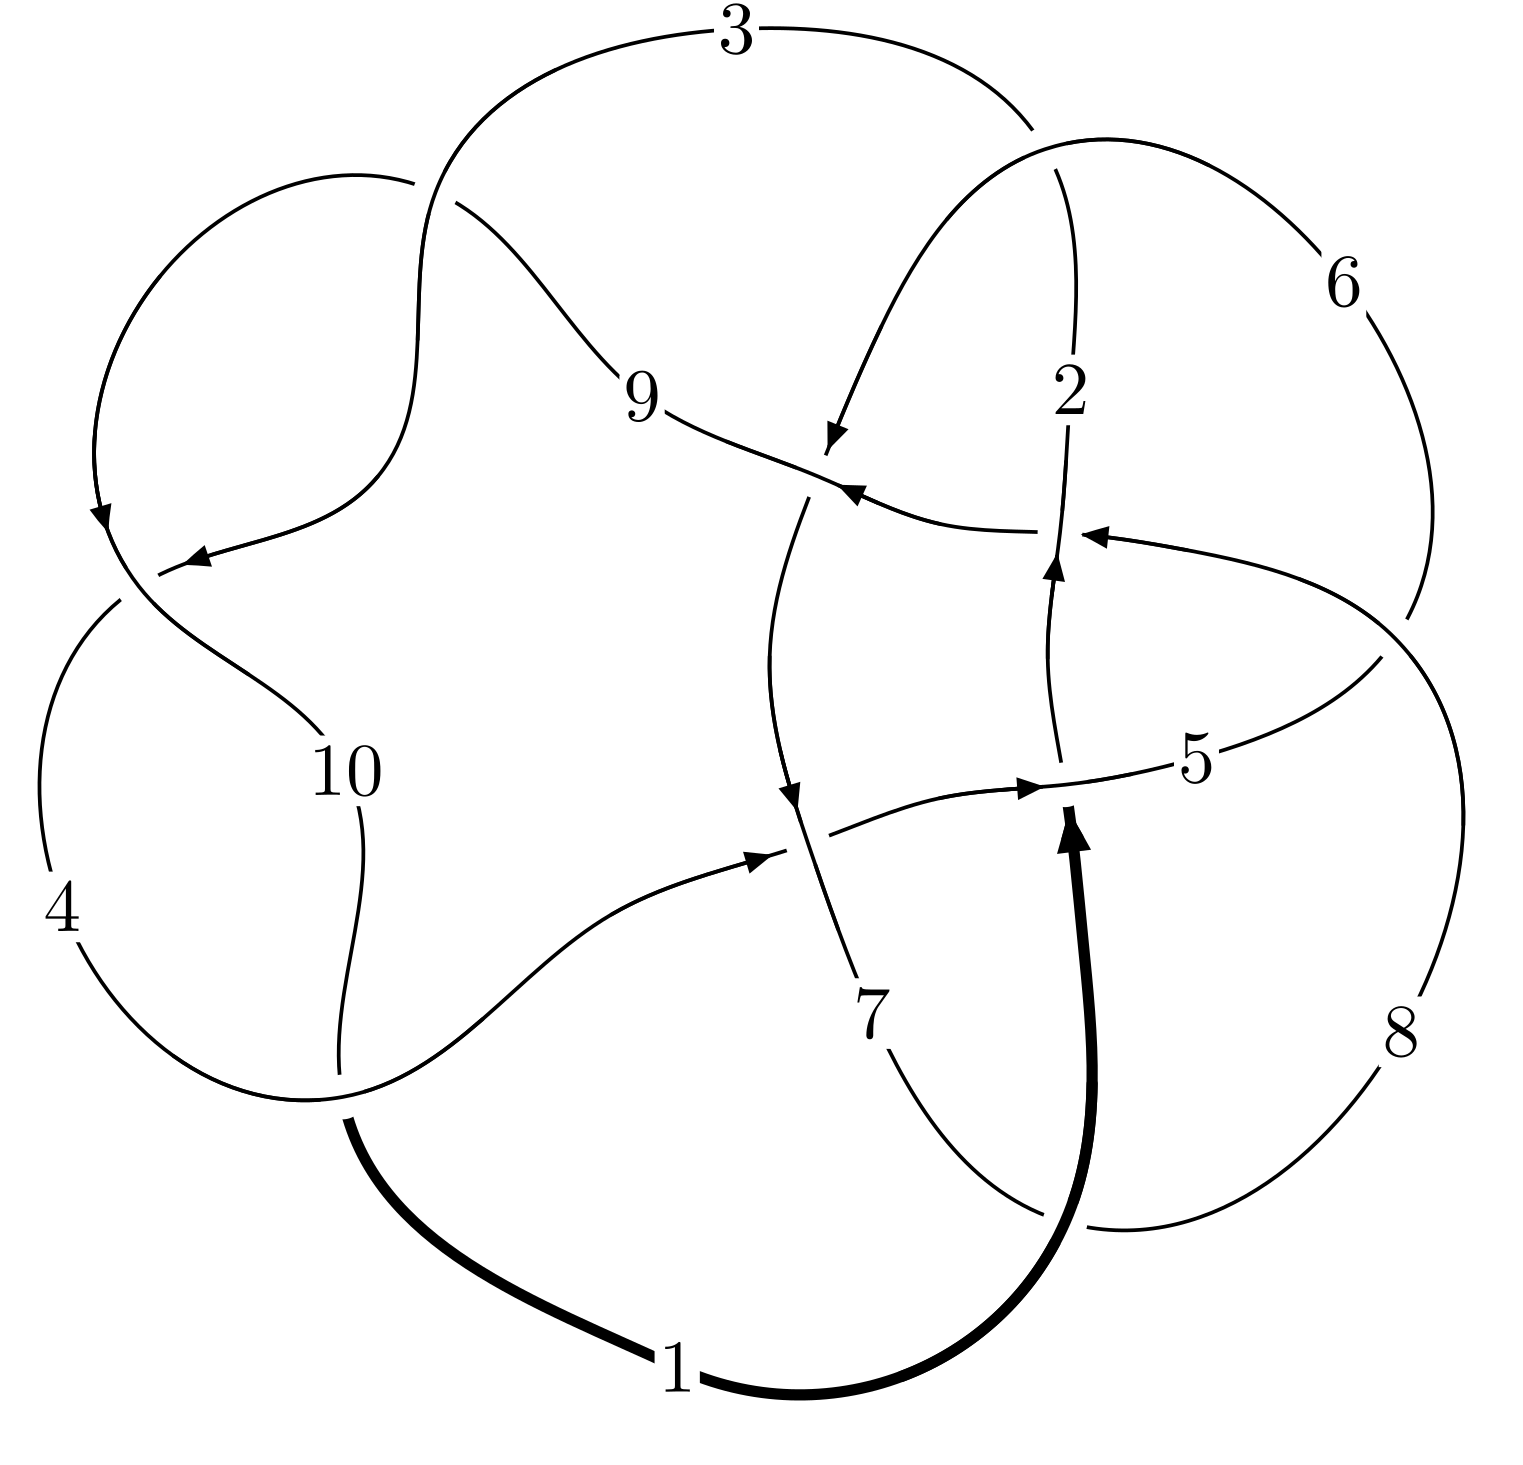
\includegraphics[width=112pt]{../../../GIT/diagram.site/Diagrams/png/196_10_112.png}\\
\ \ \ A knot diagram\footnotemark}&
\allowdisplaybreaks
\textbf{Linearized knot diagam} \\
\cline{2-2}
 &
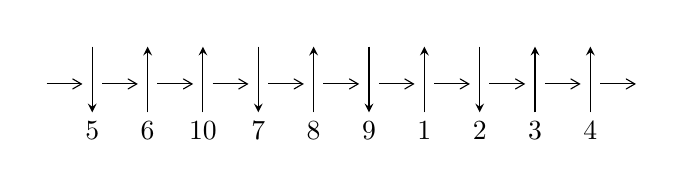
\begin{tikzpicture}[x=20pt, y=17pt]
	% nodes
	\node (C0) at (0, 0) {};
	\node (C1) at (1, 0) {};
	\node (C1U) at (1, +1) {};
	\node (C1D) at (1, -1) {5};

	\node (C2) at (2, 0) {};
	\node (C2U) at (2, +1) {};
	\node (C2D) at (2, -1) {6};

	\node (C3) at (3, 0) {};
	\node (C3U) at (3, +1) {};
	\node (C3D) at (3, -1) {10};

	\node (C4) at (4, 0) {};
	\node (C4U) at (4, +1) {};
	\node (C4D) at (4, -1) {7};

	\node (C5) at (5, 0) {};
	\node (C5U) at (5, +1) {};
	\node (C5D) at (5, -1) {8};

	\node (C6) at (6, 0) {};
	\node (C6U) at (6, +1) {};
	\node (C6D) at (6, -1) {9};

	\node (C7) at (7, 0) {};
	\node (C7U) at (7, +1) {};
	\node (C7D) at (7, -1) {1};

	\node (C8) at (8, 0) {};
	\node (C8U) at (8, +1) {};
	\node (C8D) at (8, -1) {2};

	\node (C9) at (9, 0) {};
	\node (C9U) at (9, +1) {};
	\node (C9D) at (9, -1) {3};

	\node (C10) at (10, 0) {};
	\node (C10U) at (10, +1) {};
	\node (C10D) at (10, -1) {4};
	\node (C11) at (11, 0) {};

	% arrows
	\draw[->,>={angle 60}]
	(C0) edge (C1) (C1) edge (C2) (C2) edge (C3) (C3) edge (C4) (C4) edge (C5) (C5) edge (C6) (C6) edge (C7) (C7) edge (C8) (C8) edge (C9) (C9) edge (C10) (C10) edge (C11) ;	\draw[->,>=stealth]
	(C1U) edge (C1D) (C2D) edge (C2U) (C3D) edge (C3U) (C4U) edge (C4D) (C5D) edge (C5U) (C6U) edge (C6D) (C7D) edge (C7U) (C8U) edge (C8D) (C9D) edge (C9U) (C10D) edge (C10U) ;
	\end{tikzpicture} \\
\hhline{~~} \\& 
\textbf{Solving Sequence} \\ \cline{2-2} 
 &
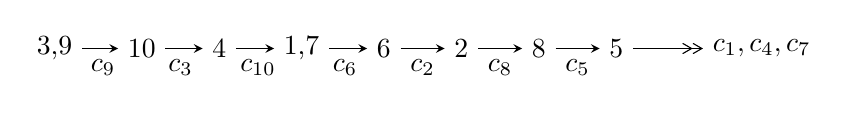
\begin{tikzpicture}[x=28pt, y=7pt]
	% node
	\node (A0) at (-1/8, 0) {3,9};
	\node (A1) at (1, 0) {10};
	\node (A2) at (2, 0) {4};
	\node (A3) at (49/16, 0) {1,7};
	\node (A4) at (33/8, 0) {6};
	\node (A5) at (41/8, 0) {2};
	\node (A6) at (49/8, 0) {8};
	\node (A7) at (57/8, 0) {5};
	\node (C1) at (1/2, -1) {$c_{9}$};
	\node (C2) at (3/2, -1) {$c_{3}$};
	\node (C3) at (5/2, -1) {$c_{10}$};
	\node (C4) at (29/8, -1) {$c_{6}$};
	\node (C5) at (37/8, -1) {$c_{2}$};
	\node (C6) at (45/8, -1) {$c_{8}$};
	\node (C7) at (53/8, -1) {$c_{5}$};
	\node (A8) at (9, 0) {$c_{1},c_{4},c_{7}$};

	% edge
	\draw[->,>=stealth]	
	(A0) edge (A1) (A1) edge (A2) (A2) edge (A3) (A3) edge (A4) (A4) edge (A5) (A5) edge (A6) (A6) edge (A7) ;
	\draw[->>,>={angle 60}]	
	(A7) edge (A8);
\end{tikzpicture} \\ 

\end{tabular} \\

\footnotetext{
The image of knot diagram is generated by the software ``\textbf{Draw programme}" developed by Andrew Bartholomew(\url{http://www.layer8.co.uk/maths/draw/index.htm\#Running-draw}), where we modified some parts for our purpose(\url{https://github.com/CATsTAILs/LinksPainter}).
}\phantom \\ \newline 
\centering \textbf{Ideals for irreducible components\footnotemark of $X_{\text{par}}$} 
 
\begin{align*}
I^u_{1}&=\langle 
-11 u^{18}+43 u^{17}+\cdots+3 b-32,\;-95 u^{18}+507 u^{17}+\cdots+21 a-761,\;u^{19}-6 u^{18}+\cdots-11 u-7\rangle \\
I^u_{2}&=\langle 
u^{14}+2 u^{13}+\cdots+b+2,\;-2 u^{14} a-2 u^{14}+\cdots-4 a-4,\\
\phantom{I^u_{2}}&\phantom{= \langle  }u^{15}+2 u^{14}-6 u^{13}-11 u^{12}+16 u^{11}+19 u^{10}-30 u^9-7 u^8+38 u^7-12 u^6-20 u^5+14 u^4-3 u^2+2 u+1\rangle \\
I^u_{3}&=\langle 
- u^4- u^3+2 u^2+b+2 u+1,\;2 u^4+u^3-5 u^2+a- u,\;u^5- u^4-3 u^3+3 u^2+1\rangle \\
I^u_{4}&=\langle 
b+1,\;a^2- a-1,\;u+1\rangle \\
\\
I^v_{1}&=\langle 
a,\;b+1,\;v+1\rangle \\
\end{align*}
\raggedright * 5 irreducible components of $\dim_{\mathbb{C}}=0$, with total 57 representations.\\
\footnotetext{All coefficients of polynomials are rational numbers. But the coefficients are sometimes approximated in decimal forms when there is not enough margin.}
\newpage
\renewcommand{\arraystretch}{1}
\centering \section*{I. $I^u_{1}= \langle -11 u^{18}+43 u^{17}+\cdots+3 b-32,\;-95 u^{18}+507 u^{17}+\cdots+21 a-761,\;u^{19}-6 u^{18}+\cdots-11 u-7 \rangle$}
\flushleft \textbf{(i) Arc colorings}\\
\begin{tabular}{m{7pt} m{180pt} m{7pt} m{180pt} }
\flushright $a_{3}=$&$\begin{pmatrix}0\\u\end{pmatrix}$ \\
\flushright $a_{9}=$&$\begin{pmatrix}1\\0\end{pmatrix}$ \\
\flushright $a_{10}=$&$\begin{pmatrix}1\\- u^2\end{pmatrix}$ \\
\flushright $a_{4}=$&$\begin{pmatrix}u\\- u^3+u\end{pmatrix}$ \\
\flushright $a_{1}=$&$\begin{pmatrix}- u^2+1\\u^4-2 u^2\end{pmatrix}$ \\
\flushright $a_{7}=$&$\begin{pmatrix}4.52381 u^{18}-24.1429 u^{17}+\cdots+85.8571 u+36.2381\\\frac{11}{3} u^{18}-\frac{43}{3} u^{17}+\cdots+\frac{64}{3} u+\frac{32}{3}\end{pmatrix}$ \\
\flushright $a_{6}=$&$\begin{pmatrix}8.19048 u^{18}-38.4762 u^{17}+\cdots+107.190 u+46.9048\\\frac{11}{3} u^{18}-\frac{43}{3} u^{17}+\cdots+\frac{64}{3} u+\frac{32}{3}\end{pmatrix}$ \\
\flushright $a_{2}=$&$\begin{pmatrix}-8.47619 u^{18}+39.5238 u^{17}+\cdots-97.4762 u-43.0952\\\frac{25}{3} u^{18}-\frac{116}{3} u^{17}+\cdots+99 u+41\end{pmatrix}$ \\
\flushright $a_{8}=$&$\begin{pmatrix}-0.809524 u^{18}+2.85714 u^{17}+\cdots+1.52381 u+0.238095\\-\frac{28}{3} u^{18}+43 u^{17}+\cdots-\frac{323}{3} u-\frac{143}{3}\end{pmatrix}$ \\
\flushright $a_{5}=$&$\begin{pmatrix}6.19048 u^{18}-30.1429 u^{17}+\cdots+87.5238 u+39.2381\\-\frac{1}{3} u^{18}+\frac{10}{3} u^{17}+\cdots-12 u-\frac{17}{3}\end{pmatrix}$\\&\end{tabular}
\flushleft \textbf{(ii) Obstruction class $= -1$}\\~\\
\flushleft \textbf{(iii) Cusp Shapes $= \frac{59}{3} u^{18}-\frac{281}{3} u^{17}+23 u^{16}+434 u^{15}-\frac{847}{3} u^{14}-\frac{2660}{3} u^{13}-22 u^{12}+\frac{5324}{3} u^{11}+1228 u^{10}-\frac{6821}{3} u^9-2347 u^8+388 u^7+\frac{9250}{3} u^6+\frac{2645}{3} u^5-1147 u^4-1166 u^3-10 u^2+\frac{733}{3} u+99$}\\~\\
\newpage\renewcommand{\arraystretch}{1}
\flushleft \textbf{(iv) u-Polynomials at the component}\newline \\
\begin{tabular}{m{50pt}|m{274pt}}
Crossings & \hspace{64pt}u-Polynomials at each crossing \\
\hline $$\begin{aligned}c_{1},c_{8}\end{aligned}$$&$\begin{aligned}
&u^{19}-2 u^{18}+\cdots-12 u^2+1
\end{aligned}$\\
\hline $$\begin{aligned}c_{2},c_{7}\end{aligned}$$&$\begin{aligned}
&u^{19}-2 u^{18}+\cdots+2 u+1
\end{aligned}$\\
\hline $$\begin{aligned}c_{3},c_{9},c_{10}\end{aligned}$$&$\begin{aligned}
&u^{19}-6 u^{18}+\cdots-11 u-7
\end{aligned}$\\
\hline $$\begin{aligned}c_{4},c_{6}\end{aligned}$$&$\begin{aligned}
&u^{19}+2 u^{18}+\cdots-2 u+1
\end{aligned}$\\
\hline $$\begin{aligned}c_{5}\end{aligned}$$&$\begin{aligned}
&u^{19}+11 u^{18}+\cdots-22 u-7
\end{aligned}$\\
\hline
\end{tabular}\\~\\
\newpage\renewcommand{\arraystretch}{1}
\flushleft \textbf{(v) Riley Polynomials at the component}\newline \\
\begin{tabular}{m{50pt}|m{274pt}}
Crossings & \hspace{64pt}Riley Polynomials at each crossing \\
\hline $$\begin{aligned}c_{1},c_{8}\end{aligned}$$&$\begin{aligned}
&y^{19}-12 y^{18}+\cdots+24 y-1
\end{aligned}$\\
\hline $$\begin{aligned}c_{2},c_{7}\end{aligned}$$&$\begin{aligned}
&y^{19}-6 y^{18}+\cdots+6 y-1
\end{aligned}$\\
\hline $$\begin{aligned}c_{3},c_{9},c_{10}\end{aligned}$$&$\begin{aligned}
&y^{19}-22 y^{18}+\cdots+331 y-49
\end{aligned}$\\
\hline $$\begin{aligned}c_{4},c_{6}\end{aligned}$$&$\begin{aligned}
&y^{19}-2 y^{18}+\cdots+18 y-1
\end{aligned}$\\
\hline $$\begin{aligned}c_{5}\end{aligned}$$&$\begin{aligned}
&y^{19}- y^{18}+\cdots+316 y-49
\end{aligned}$\\
\hline
\end{tabular}\\~\\
\newpage\flushleft \textbf{(vi) Complex Volumes and Cusp Shapes}
$$\begin{array}{c|c|c}  
\text{Solutions to }I^u_{1}& \I (\text{vol} + \sqrt{-1}CS) & \text{Cusp shape}\\
 \hline 
\begin{aligned}
u &= -0.650742 + 0.795961 I \\
a &= \phantom{-}0.354047 - 0.615330 I \\
b &= \phantom{-}0.971206 + 0.919721 I\end{aligned}
 & \phantom{-}0.21692 - 10.80920 I & \phantom{-}2.85095 + 8.95586 I \\ \hline\begin{aligned}
u &= -0.650742 - 0.795961 I \\
a &= \phantom{-}0.354047 + 0.615330 I \\
b &= \phantom{-}0.971206 - 0.919721 I\end{aligned}
 & \phantom{-}0.21692 + 10.80920 I & \phantom{-}2.85095 - 8.95586 I \\ \hline\begin{aligned}
u &= -0.438994 + 0.966374 I \\
a &= -0.257963 - 0.341691 I \\
b &= \phantom{-}0.542166 - 0.571410 I\end{aligned}
 & -0.47646 + 5.13597 I & \phantom{-}2.04643 - 8.91772 I \\ \hline\begin{aligned}
u &= -0.438994 - 0.966374 I \\
a &= -0.257963 + 0.341691 I \\
b &= \phantom{-}0.542166 + 0.571410 I\end{aligned}
 & -0.47646 - 5.13597 I & \phantom{-}2.04643 + 8.91772 I \\ \hline\begin{aligned}
u &= -0.500281 + 0.484136 I \\
a &= -0.276043 + 1.168470 I \\
b &= -0.989225 - 0.870492 I\end{aligned}
 & -1.71464 - 3.32825 I & -3.18882 + 7.99623 I \\ \hline\begin{aligned}
u &= -0.500281 - 0.484136 I \\
a &= -0.276043 - 1.168470 I \\
b &= -0.989225 + 0.870492 I\end{aligned}
 & -1.71464 + 3.32825 I & -3.18882 - 7.99623 I \\ \hline\begin{aligned}
u &= \phantom{-}1.320090 + 0.044695 I \\
a &= \phantom{-}0.592095 + 1.229420 I \\
b &= -0.158877 - 0.560433 I\end{aligned}
 & \phantom{-}2.62449 - 0.38341 I & \phantom{-}2.28736 + 1.27302 I \\ \hline\begin{aligned}
u &= \phantom{-}1.320090 - 0.044695 I \\
a &= \phantom{-}0.592095 - 1.229420 I \\
b &= -0.158877 + 0.560433 I\end{aligned}
 & \phantom{-}2.62449 + 0.38341 I & \phantom{-}2.28736 - 1.27302 I \\ \hline\begin{aligned}
u &= \phantom{-}0.612375\phantom{ +0.000000I} \\
a &= \phantom{-}0.930010\phantom{ +0.000000I} \\
b &= \phantom{-}0.220758\phantom{ +0.000000I}\end{aligned}
 & \phantom{-}1.15807\phantom{ +0.000000I} & \phantom{-}8.48700\phantom{ +0.000000I} \\ \hline\begin{aligned}
u &= -1.43114\phantom{ +0.000000I} \\
a &= \phantom{-}0.461846\phantom{ +0.000000I} \\
b &= -1.60691\phantom{ +0.000000I}\end{aligned}
 & \phantom{-}3.44527\phantom{ +0.000000I} & \phantom{-}2.15800\phantom{ +0.000000I}\\
 \hline 
 \end{array}$$\newpage$$\begin{array}{c|c|c}  
\text{Solutions to }I^u_{1}& \I (\text{vol} + \sqrt{-1}CS) & \text{Cusp shape}\\
 \hline 
\begin{aligned}
u &= -0.397187 + 0.334084 I \\
a &= \phantom{-}0.957646 + 0.804912 I \\
b &= -0.907078 + 0.217237 I\end{aligned}
 & -1.91282 + 0.23550 I & -3.85755 + 0.64166 I \\ \hline\begin{aligned}
u &= -0.397187 - 0.334084 I \\
a &= \phantom{-}0.957646 - 0.804912 I \\
b &= -0.907078 - 0.217237 I\end{aligned}
 & -1.91282 - 0.23550 I & -3.85755 - 0.64166 I \\ \hline\begin{aligned}
u &= \phantom{-}1.52853 + 0.13991 I \\
a &= \phantom{-}0.49931 - 2.07085 I \\
b &= -0.98962 + 1.48876 I\end{aligned}
 & \phantom{-}5.05013 + 5.56057 I & -1.07165 - 5.51845 I \\ \hline\begin{aligned}
u &= \phantom{-}1.52853 - 0.13991 I \\
a &= \phantom{-}0.49931 + 2.07085 I \\
b &= -0.98962 - 1.48876 I\end{aligned}
 & \phantom{-}5.05013 - 5.56057 I & -1.07165 + 5.51845 I \\ \hline\begin{aligned}
u &= -1.55827\phantom{ +0.000000I} \\
a &= -0.243774\phantom{ +0.000000I} \\
b &= \phantom{-}0.971797\phantom{ +0.000000I}\end{aligned}
 & \phantom{-}8.51485\phantom{ +0.000000I} & \phantom{-}10.8570\phantom{ +0.000000I} \\ \hline\begin{aligned}
u &= \phantom{-}1.58255 + 0.26743 I \\
a &= -0.25739 + 1.68674 I \\
b &= \phantom{-}1.19555 - 1.28537 I\end{aligned}
 & \phantom{-}7.5458 + 14.7559 I & \phantom{-}5.72071 - 7.88264 I \\ \hline\begin{aligned}
u &= \phantom{-}1.58255 - 0.26743 I \\
a &= -0.25739 - 1.68674 I \\
b &= \phantom{-}1.19555 + 1.28537 I\end{aligned}
 & \phantom{-}7.5458 - 14.7559 I & \phantom{-}5.72071 + 7.88264 I \\ \hline\begin{aligned}
u &= \phantom{-}1.74455 + 0.26523 I \\
a &= \phantom{-}0.099974 - 0.506108 I \\
b &= -0.456945 + 0.555778 I\end{aligned}
 & \phantom{-}6.78146 + 0.51735 I & \phantom{-}9.96153 - 9.39104 I \\ \hline\begin{aligned}
u &= \phantom{-}1.74455 - 0.26523 I \\
a &= \phantom{-}0.099974 + 0.506108 I \\
b &= -0.456945 - 0.555778 I\end{aligned}
 & \phantom{-}6.78146 - 0.51735 I & \phantom{-}9.96153 + 9.39104 I\\
 \hline 
 \end{array}$$\newpage\newpage\renewcommand{\arraystretch}{1}
\centering \section*{II. $I^u_{2}= \langle u^{14}+2 u^{13}+\cdots+b+2,\;-2 u^{14} a-2 u^{14}+\cdots-4 a-4,\;u^{15}+2 u^{14}+\cdots+2 u+1 \rangle$}
\flushleft \textbf{(i) Arc colorings}\\
\begin{tabular}{m{7pt} m{180pt} m{7pt} m{180pt} }
\flushright $a_{3}=$&$\begin{pmatrix}0\\u\end{pmatrix}$ \\
\flushright $a_{9}=$&$\begin{pmatrix}1\\0\end{pmatrix}$ \\
\flushright $a_{10}=$&$\begin{pmatrix}1\\- u^2\end{pmatrix}$ \\
\flushright $a_{4}=$&$\begin{pmatrix}u\\- u^3+u\end{pmatrix}$ \\
\flushright $a_{1}=$&$\begin{pmatrix}- u^2+1\\u^4-2 u^2\end{pmatrix}$ \\
\flushright $a_{7}=$&$\begin{pmatrix}a\\- u^{14}-2 u^{13}+\cdots- a u-2\end{pmatrix}$ \\
\flushright $a_{6}=$&$\begin{pmatrix}- u^{14}-2 u^{13}+\cdots+a-2\\- u^{14}-2 u^{13}+\cdots- a u-2\end{pmatrix}$ \\
\flushright $a_{2}=$&$\begin{pmatrix}- u^{13}- u^{12}+\cdots+a-3 u\\- u^{14} a- u^{13} a+\cdots- a-1\end{pmatrix}$ \\
\flushright $a_{8}=$&$\begin{pmatrix}- u^{13}- u^{12}+\cdots+a-1\\- u^{14}- u^{13}+\cdots- u-2\end{pmatrix}$ \\
\flushright $a_{5}=$&$\begin{pmatrix}u^{14} a- u^{14}+\cdots+2 a- u\\1\end{pmatrix}$\\&\end{tabular}
\flushleft \textbf{(ii) Obstruction class $= -1$}\\~\\
\flushleft \textbf{(iii) Cusp Shapes $= 11 u^{14}+9 u^{13}-77 u^{12}-34 u^{11}+218 u^{10}-21 u^9-319 u^8+224 u^7+214 u^6-298 u^5+14 u^4+132 u^3-60 u^2-5 u+23$}\\~\\
\newpage\renewcommand{\arraystretch}{1}
\flushleft \textbf{(iv) u-Polynomials at the component}\newline \\
\begin{tabular}{m{50pt}|m{274pt}}
Crossings & \hspace{64pt}u-Polynomials at each crossing \\
\hline $$\begin{aligned}c_{1},c_{8}\end{aligned}$$&$\begin{aligned}
&u^{30}+2 u^{28}+\cdots+7 u+1
\end{aligned}$\\
\hline $$\begin{aligned}c_{2},c_{7}\end{aligned}$$&$\begin{aligned}
&u^{30}-4 u^{28}+\cdots-37 u+43
\end{aligned}$\\
\hline $$\begin{aligned}c_{3},c_{9},c_{10}\end{aligned}$$&$\begin{aligned}
&(u^{15}+2 u^{14}+\cdots+2 u+1)^{2}
\end{aligned}$\\
\hline $$\begin{aligned}c_{4},c_{6}\end{aligned}$$&$\begin{aligned}
&u^{30}-3 u^{29}+\cdots-42 u+7
\end{aligned}$\\
\hline $$\begin{aligned}c_{5}\end{aligned}$$&$\begin{aligned}
&(u^{15}-7 u^{14}+\cdots+3 u-2)^{2}
\end{aligned}$\\
\hline
\end{tabular}\\~\\
\newpage\renewcommand{\arraystretch}{1}
\flushleft \textbf{(v) Riley Polynomials at the component}\newline \\
\begin{tabular}{m{50pt}|m{274pt}}
Crossings & \hspace{64pt}Riley Polynomials at each crossing \\
\hline $$\begin{aligned}c_{1},c_{8}\end{aligned}$$&$\begin{aligned}
&y^{30}+4 y^{29}+\cdots-19 y+1
\end{aligned}$\\
\hline $$\begin{aligned}c_{2},c_{7}\end{aligned}$$&$\begin{aligned}
&y^{30}-8 y^{29}+\cdots-32587 y+1849
\end{aligned}$\\
\hline $$\begin{aligned}c_{3},c_{9},c_{10}\end{aligned}$$&$\begin{aligned}
&(y^{15}-16 y^{14}+\cdots+10 y-1)^{2}
\end{aligned}$\\
\hline $$\begin{aligned}c_{4},c_{6}\end{aligned}$$&$\begin{aligned}
&y^{30}+13 y^{29}+\cdots+182 y+49
\end{aligned}$\\
\hline $$\begin{aligned}c_{5}\end{aligned}$$&$\begin{aligned}
&(y^{15}-3 y^{14}+\cdots+37 y-4)^{2}
\end{aligned}$\\
\hline
\end{tabular}\\~\\
\newpage\flushleft \textbf{(vi) Complex Volumes and Cusp Shapes}
$$\begin{array}{c|c|c}  
\text{Solutions to }I^u_{2}& \I (\text{vol} + \sqrt{-1}CS) & \text{Cusp shape}\\
 \hline 
\begin{aligned}
u &= \phantom{-}0.564527 + 0.799929 I \\
a &= \phantom{-}0.618356 + 0.354320 I \\
b &= \phantom{-}0.554999 - 0.686515 I\end{aligned}
 & \phantom{-}2.03837 + 2.66927 I & \phantom{-}9.65376 - 4.84373 I \\ \hline\begin{aligned}
u &= \phantom{-}0.564527 + 0.799929 I \\
a &= -0.180396 - 0.172783 I \\
b &= -0.148347 + 0.802094 I\end{aligned}
 & \phantom{-}2.03837 + 2.66927 I & \phantom{-}9.65376 - 4.84373 I \\ \hline\begin{aligned}
u &= \phantom{-}0.564527 - 0.799929 I \\
a &= \phantom{-}0.618356 - 0.354320 I \\
b &= \phantom{-}0.554999 + 0.686515 I\end{aligned}
 & \phantom{-}2.03837 - 2.66927 I & \phantom{-}9.65376 + 4.84373 I \\ \hline\begin{aligned}
u &= \phantom{-}0.564527 - 0.799929 I \\
a &= -0.180396 + 0.172783 I \\
b &= -0.148347 - 0.802094 I\end{aligned}
 & \phantom{-}2.03837 - 2.66927 I & \phantom{-}9.65376 + 4.84373 I \\ \hline\begin{aligned}
u &= \phantom{-}0.860038 + 0.294980 I \\
a &= \phantom{-}1.344360 - 0.145933 I \\
b &= -0.576437 - 0.370669 I\end{aligned}
 & \phantom{-}0.620973 - 0.239040 I & \phantom{-}7.64024 + 3.49944 I \\ \hline\begin{aligned}
u &= \phantom{-}0.860038 + 0.294980 I \\
a &= \phantom{-}0.467288 + 0.091114 I \\
b &= \phantom{-}0.940505 - 0.025509 I\end{aligned}
 & \phantom{-}0.620973 - 0.239040 I & \phantom{-}7.64024 + 3.49944 I \\ \hline\begin{aligned}
u &= \phantom{-}0.860038 - 0.294980 I \\
a &= \phantom{-}1.344360 + 0.145933 I \\
b &= -0.576437 + 0.370669 I\end{aligned}
 & \phantom{-}0.620973 + 0.239040 I & \phantom{-}7.64024 - 3.49944 I \\ \hline\begin{aligned}
u &= \phantom{-}0.860038 - 0.294980 I \\
a &= \phantom{-}0.467288 - 0.091114 I \\
b &= \phantom{-}0.940505 + 0.025509 I\end{aligned}
 & \phantom{-}0.620973 + 0.239040 I & \phantom{-}7.64024 - 3.49944 I \\ \hline\begin{aligned}
u &= \phantom{-}0.239953 + 0.580457 I \\
a &= -0.446760 - 0.059168 I \\
b &= -0.908941 + 1.005900 I\end{aligned}
 & -1.25960 + 3.60373 I & -3.55671 - 7.52468 I \\ \hline\begin{aligned}
u &= \phantom{-}0.239953 + 0.580457 I \\
a &= \phantom{-}0.85432 + 1.67566 I \\
b &= \phantom{-}0.632582 - 0.043404 I\end{aligned}
 & -1.25960 + 3.60373 I & -3.55671 - 7.52468 I\\
 \hline 
 \end{array}$$\newpage$$\begin{array}{c|c|c}  
\text{Solutions to }I^u_{2}& \I (\text{vol} + \sqrt{-1}CS) & \text{Cusp shape}\\
 \hline 
\begin{aligned}
u &= \phantom{-}0.239953 - 0.580457 I \\
a &= -0.446760 + 0.059168 I \\
b &= -0.908941 - 1.005900 I\end{aligned}
 & -1.25960 - 3.60373 I & -3.55671 + 7.52468 I \\ \hline\begin{aligned}
u &= \phantom{-}0.239953 - 0.580457 I \\
a &= \phantom{-}0.85432 - 1.67566 I \\
b &= \phantom{-}0.632582 + 0.043404 I\end{aligned}
 & -1.25960 - 3.60373 I & -3.55671 + 7.52468 I \\ \hline\begin{aligned}
u &= -1.42712 + 0.14742 I \\
a &= -0.17362 - 1.66530 I \\
b &= \phantom{-}0.195570 + 0.362588 I\end{aligned}
 & \phantom{-}4.10336 - 6.07313 I & \phantom{-}1.68774 + 6.92177 I \\ \hline\begin{aligned}
u &= -1.42712 + 0.14742 I \\
a &= \phantom{-}0.38365 + 2.08559 I \\
b &= -1.15734 - 1.68991 I\end{aligned}
 & \phantom{-}4.10336 - 6.07313 I & \phantom{-}1.68774 + 6.92177 I \\ \hline\begin{aligned}
u &= -1.42712 - 0.14742 I \\
a &= -0.17362 + 1.66530 I \\
b &= \phantom{-}0.195570 - 0.362588 I\end{aligned}
 & \phantom{-}4.10336 + 6.07313 I & \phantom{-}1.68774 - 6.92177 I \\ \hline\begin{aligned}
u &= -1.42712 - 0.14742 I \\
a &= \phantom{-}0.38365 - 2.08559 I \\
b &= -1.15734 + 1.68991 I\end{aligned}
 & \phantom{-}4.10336 + 6.07313 I & \phantom{-}1.68774 - 6.92177 I \\ \hline\begin{aligned}
u &= \phantom{-}1.49768 + 0.04419 I \\
a &= -0.20828 - 1.77267 I \\
b &= -0.809632 + 1.029070 I\end{aligned}
 & \phantom{-}7.81267 + 4.54595 I & \phantom{-}9.44858 - 4.92517 I \\ \hline\begin{aligned}
u &= \phantom{-}1.49768 + 0.04419 I \\
a &= -0.75346 - 1.96166 I \\
b &= \phantom{-}1.19533 + 1.83190 I\end{aligned}
 & \phantom{-}7.81267 + 4.54595 I & \phantom{-}9.44858 - 4.92517 I \\ \hline\begin{aligned}
u &= \phantom{-}1.49768 - 0.04419 I \\
a &= -0.20828 + 1.77267 I \\
b &= -0.809632 - 1.029070 I\end{aligned}
 & \phantom{-}7.81267 - 4.54595 I & \phantom{-}9.44858 + 4.92517 I \\ \hline\begin{aligned}
u &= \phantom{-}1.49768 - 0.04419 I \\
a &= -0.75346 + 1.96166 I \\
b &= \phantom{-}1.19533 - 1.83190 I\end{aligned}
 & \phantom{-}7.81267 - 4.54595 I & \phantom{-}9.44858 + 4.92517 I\\
 \hline 
 \end{array}$$\newpage$$\begin{array}{c|c|c}  
\text{Solutions to }I^u_{2}& \I (\text{vol} + \sqrt{-1}CS) & \text{Cusp shape}\\
 \hline 
\begin{aligned}
u &= -1.54349\phantom{ +0.000000I} \\
a &= -0.239030 + 0.599706 I \\
b &= \phantom{-}0.938402 - 0.503082 I\end{aligned}
 & \phantom{-}8.47953\phantom{ +0.000000I} & \phantom{-}10.2010\phantom{ +0.000000I} \\ \hline\begin{aligned}
u &= -1.54349\phantom{ +0.000000I} \\
a &= -0.239030 - 0.599706 I \\
b &= \phantom{-}0.938402 + 0.503082 I\end{aligned}
 & \phantom{-}8.47953\phantom{ +0.000000I} & \phantom{-}10.2010\phantom{ +0.000000I} \\ \hline\begin{aligned}
u &= -0.406537 + 0.119542 I \\
a &= \phantom{-}1.03173 + 0.97861 I \\
b &= \phantom{-}0.502233 - 1.320460 I\end{aligned}
 & \phantom{-}1.41571 - 3.90370 I & \phantom{-}10.38515 + 7.89648 I \\ \hline\begin{aligned}
u &= -0.406537 + 0.119542 I \\
a &= -2.55257 + 2.38070 I \\
b &= -0.382424 - 0.882051 I\end{aligned}
 & \phantom{-}1.41571 - 3.90370 I & \phantom{-}10.38515 + 7.89648 I \\ \hline\begin{aligned}
u &= -0.406537 - 0.119542 I \\
a &= \phantom{-}1.03173 - 0.97861 I \\
b &= \phantom{-}0.502233 + 1.320460 I\end{aligned}
 & \phantom{-}1.41571 + 3.90370 I & \phantom{-}10.38515 - 7.89648 I \\ \hline\begin{aligned}
u &= -0.406537 - 0.119542 I \\
a &= -2.55257 - 2.38070 I \\
b &= -0.382424 + 0.882051 I\end{aligned}
 & \phantom{-}1.41571 + 3.90370 I & \phantom{-}10.38515 - 7.89648 I \\ \hline\begin{aligned}
u &= -1.55680 + 0.27188 I \\
a &= \phantom{-}0.037420 - 1.346330 I \\
b &= \phantom{-}0.959638 + 0.986410 I\end{aligned}
 & \phantom{-}8.99262 - 6.60915 I & \phantom{-}9.14063 + 5.69443 I \\ \hline\begin{aligned}
u &= -1.55680 + 0.27188 I \\
a &= -0.183014 + 1.386800 I \\
b &= -0.436143 - 1.307360 I\end{aligned}
 & \phantom{-}8.99262 - 6.60915 I & \phantom{-}9.14063 + 5.69443 I \\ \hline\begin{aligned}
u &= -1.55680 - 0.27188 I \\
a &= \phantom{-}0.037420 + 1.346330 I \\
b &= \phantom{-}0.959638 - 0.986410 I\end{aligned}
 & \phantom{-}8.99262 + 6.60915 I & \phantom{-}9.14063 - 5.69443 I \\ \hline\begin{aligned}
u &= -1.55680 - 0.27188 I \\
a &= -0.183014 - 1.386800 I \\
b &= -0.436143 + 1.307360 I\end{aligned}
 & \phantom{-}8.99262 + 6.60915 I & \phantom{-}9.14063 - 5.69443 I\\
 \hline 
 \end{array}$$\newpage\newpage\renewcommand{\arraystretch}{1}
\centering \section*{III. $I^u_{3}= \langle - u^4- u^3+2 u^2+b+2 u+1,\;2 u^4+u^3-5 u^2+a- u,\;u^5- u^4-3 u^3+3 u^2+1 \rangle$}
\flushleft \textbf{(i) Arc colorings}\\
\begin{tabular}{m{7pt} m{180pt} m{7pt} m{180pt} }
\flushright $a_{3}=$&$\begin{pmatrix}0\\u\end{pmatrix}$ \\
\flushright $a_{9}=$&$\begin{pmatrix}1\\0\end{pmatrix}$ \\
\flushright $a_{10}=$&$\begin{pmatrix}1\\- u^2\end{pmatrix}$ \\
\flushright $a_{4}=$&$\begin{pmatrix}u\\- u^3+u\end{pmatrix}$ \\
\flushright $a_{1}=$&$\begin{pmatrix}- u^2+1\\u^4-2 u^2\end{pmatrix}$ \\
\flushright $a_{7}=$&$\begin{pmatrix}-2 u^4- u^3+5 u^2+u\\u^4+u^3-2 u^2-2 u-1\end{pmatrix}$ \\
\flushright $a_{6}=$&$\begin{pmatrix}- u^4+3 u^2- u-1\\u^4+u^3-2 u^2-2 u-1\end{pmatrix}$ \\
\flushright $a_{2}=$&$\begin{pmatrix}- u^4+2 u^2- u+2\\u^4-3 u^2+u\end{pmatrix}$ \\
\flushright $a_{8}=$&$\begin{pmatrix}- u^4+3 u^2- u\\u^3-2 u\end{pmatrix}$ \\
\flushright $a_{5}=$&$\begin{pmatrix}- u^4+2 u^2- u\\u^4-2 u^2\end{pmatrix}$\\&\end{tabular}
\flushleft \textbf{(ii) Obstruction class $= 1$}\\~\\
\flushleft \textbf{(iii) Cusp Shapes $= -4 u^4-7 u^3+10 u^2+14 u+6$}\\~\\
\newpage\renewcommand{\arraystretch}{1}
\flushleft \textbf{(iv) u-Polynomials at the component}\newline \\
\begin{tabular}{m{50pt}|m{274pt}}
Crossings & \hspace{64pt}u-Polynomials at each crossing \\
\hline $$\begin{aligned}c_{1},c_{8}\end{aligned}$$&$\begin{aligned}
&u^5+u^4+u^2+u+1
\end{aligned}$\\
\hline $$\begin{aligned}c_{2},c_{7}\end{aligned}$$&$\begin{aligned}
&u^5- u^4+u^3+u-1
\end{aligned}$\\
\hline $$\begin{aligned}c_{3}\end{aligned}$$&$\begin{aligned}
&u^5+u^4-3 u^3-3 u^2-1
\end{aligned}$\\
\hline $$\begin{aligned}c_{4},c_{6}\end{aligned}$$&$\begin{aligned}
&u^5- u^4+3 u^3+u+1
\end{aligned}$\\
\hline $$\begin{aligned}c_{5}\end{aligned}$$&$\begin{aligned}
&u^5+4 u^4+9 u^3+13 u^2+11 u+5
\end{aligned}$\\
\hline $$\begin{aligned}c_{9},c_{10}\end{aligned}$$&$\begin{aligned}
&u^5- u^4-3 u^3+3 u^2+1
\end{aligned}$\\
\hline
\end{tabular}\\~\\
\newpage\renewcommand{\arraystretch}{1}
\flushleft \textbf{(v) Riley Polynomials at the component}\newline \\
\begin{tabular}{m{50pt}|m{274pt}}
Crossings & \hspace{64pt}Riley Polynomials at each crossing \\
\hline $$\begin{aligned}c_{1},c_{8}\end{aligned}$$&$\begin{aligned}
&y^5- y^4-3 y^2- y-1
\end{aligned}$\\
\hline $$\begin{aligned}c_{2},c_{7}\end{aligned}$$&$\begin{aligned}
&y^5+y^4+3 y^3+y-1
\end{aligned}$\\
\hline $$\begin{aligned}c_{3},c_{9},c_{10}\end{aligned}$$&$\begin{aligned}
&y^5-7 y^4+15 y^3-7 y^2-6 y-1
\end{aligned}$\\
\hline $$\begin{aligned}c_{4},c_{6}\end{aligned}$$&$\begin{aligned}
&y^5+5 y^4+11 y^3+8 y^2+y-1
\end{aligned}$\\
\hline $$\begin{aligned}c_{5}\end{aligned}$$&$\begin{aligned}
&y^5+2 y^4- y^3-11 y^2-9 y-25
\end{aligned}$\\
\hline
\end{tabular}\\~\\
\newpage\flushleft \textbf{(vi) Complex Volumes and Cusp Shapes}
$$\begin{array}{c|c|c}  
\text{Solutions to }I^u_{3}& \I (\text{vol} + \sqrt{-1}CS) & \text{Cusp shape}\\
 \hline 
\begin{aligned}
u &= \phantom{-}1.48162 + 0.12936 I \\
a &= -0.00174 - 2.14399 I \\
b &= -0.54328 + 1.49449 I\end{aligned}
 & \phantom{-}6.00251 + 5.77307 I & \phantom{-}7.88552 - 6.98438 I \\ \hline\begin{aligned}
u &= \phantom{-}1.48162 - 0.12936 I \\
a &= -0.00174 + 2.14399 I \\
b &= -0.54328 - 1.49449 I\end{aligned}
 & \phantom{-}6.00251 - 5.77307 I & \phantom{-}7.88552 + 6.98438 I \\ \hline\begin{aligned}
u &= -0.099006 + 0.496292 I \\
a &= -1.44626 + 0.01961 I \\
b &= -0.210516 - 0.857202 I\end{aligned}
 & \phantom{-}0.38751 - 3.74061 I & \phantom{-}1.55846 + 6.53295 I \\ \hline\begin{aligned}
u &= -0.099006 - 0.496292 I \\
a &= -1.44626 - 0.01961 I \\
b &= -0.210516 + 0.857202 I\end{aligned}
 & \phantom{-}0.38751 + 3.74061 I & \phantom{-}1.55846 - 6.53295 I \\ \hline\begin{aligned}
u &= -1.76524\phantom{ +0.000000I} \\
a &= -0.103987\phantom{ +0.000000I} \\
b &= \phantom{-}0.507589\phantom{ +0.000000I}\end{aligned}
 & \phantom{-}6.95916\phantom{ +0.000000I} & \phantom{-}12.1120\phantom{ +0.000000I}\\
 \hline 
 \end{array}$$\newpage\newpage\renewcommand{\arraystretch}{1}
\centering \section*{IV. $I^u_{4}= \langle b+1,\;a^2- a-1,\;u+1 \rangle$}
\flushleft \textbf{(i) Arc colorings}\\
\begin{tabular}{m{7pt} m{180pt} m{7pt} m{180pt} }
\flushright $a_{3}=$&$\begin{pmatrix}0\\-1\end{pmatrix}$ \\
\flushright $a_{9}=$&$\begin{pmatrix}1\\0\end{pmatrix}$ \\
\flushright $a_{10}=$&$\begin{pmatrix}1\\-1\end{pmatrix}$ \\
\flushright $a_{4}=$&$\begin{pmatrix}-1\\0\end{pmatrix}$ \\
\flushright $a_{1}=$&$\begin{pmatrix}0\\-1\end{pmatrix}$ \\
\flushright $a_{7}=$&$\begin{pmatrix}a\\-1\end{pmatrix}$ \\
\flushright $a_{6}=$&$\begin{pmatrix}a-1\\-1\end{pmatrix}$ \\
\flushright $a_{2}=$&$\begin{pmatrix}- a+2\\- a\end{pmatrix}$ \\
\flushright $a_{8}=$&$\begin{pmatrix}a\\- a-1\end{pmatrix}$ \\
\flushright $a_{5}=$&$\begin{pmatrix}a-1\\-1\end{pmatrix}$\\&\end{tabular}
\flushleft \textbf{(ii) Obstruction class $= 1$}\\~\\
\flushleft \textbf{(iii) Cusp Shapes $= -5$}\\~\\
\newpage\renewcommand{\arraystretch}{1}
\flushleft \textbf{(iv) u-Polynomials at the component}\newline \\
\begin{tabular}{m{50pt}|m{274pt}}
Crossings & \hspace{64pt}u-Polynomials at each crossing \\
\hline $$\begin{aligned}c_{1},c_{2},c_{7}\\c_{8}\end{aligned}$$&$\begin{aligned}
&u^2+u-1
\end{aligned}$\\
\hline $$\begin{aligned}c_{3},c_{4},c_{6}\end{aligned}$$&$\begin{aligned}
&(u-1)^2
\end{aligned}$\\
\hline $$\begin{aligned}c_{5}\end{aligned}$$&$\begin{aligned}
&u^2
\end{aligned}$\\
\hline $$\begin{aligned}c_{9},c_{10}\end{aligned}$$&$\begin{aligned}
&(u+1)^2
\end{aligned}$\\
\hline
\end{tabular}\\~\\
\newpage\renewcommand{\arraystretch}{1}
\flushleft \textbf{(v) Riley Polynomials at the component}\newline \\
\begin{tabular}{m{50pt}|m{274pt}}
Crossings & \hspace{64pt}Riley Polynomials at each crossing \\
\hline $$\begin{aligned}c_{1},c_{2},c_{7}\\c_{8}\end{aligned}$$&$\begin{aligned}
&y^2-3 y+1
\end{aligned}$\\
\hline $$\begin{aligned}c_{3},c_{4},c_{6}\\c_{9},c_{10}\end{aligned}$$&$\begin{aligned}
&(y-1)^2
\end{aligned}$\\
\hline $$\begin{aligned}c_{5}\end{aligned}$$&$\begin{aligned}
&y^2
\end{aligned}$\\
\hline
\end{tabular}\\~\\
\newpage\flushleft \textbf{(vi) Complex Volumes and Cusp Shapes}
$$\begin{array}{c|c|c}  
\text{Solutions to }I^u_{4}& \I (\text{vol} + \sqrt{-1}CS) & \text{Cusp shape}\\
 \hline 
\begin{aligned}
u &= -1.00000\phantom{ +0.000000I} \\
a &= -0.618034\phantom{ +0.000000I} \\
b &= -1.00000\phantom{ +0.000000I}\end{aligned}
 & \phantom{-0.000000 } 0 & -5.00000\phantom{ +0.000000I} \\ \hline\begin{aligned}
u &= -1.00000\phantom{ +0.000000I} \\
a &= \phantom{-}1.61803\phantom{ +0.000000I} \\
b &= -1.00000\phantom{ +0.000000I}\end{aligned}
 & \phantom{-0.000000 } 0 & -5.00000\phantom{ +0.000000I}\\
 \hline 
 \end{array}$$\newpage\newpage\renewcommand{\arraystretch}{1}
\centering \section*{V. $I^v_{1}= \langle a,\;b+1,\;v+1 \rangle$}
\flushleft \textbf{(i) Arc colorings}\\
\begin{tabular}{m{7pt} m{180pt} m{7pt} m{180pt} }
\flushright $a_{3}=$&$\begin{pmatrix}-1\\0\end{pmatrix}$ \\
\flushright $a_{9}=$&$\begin{pmatrix}1\\0\end{pmatrix}$ \\
\flushright $a_{10}=$&$\begin{pmatrix}1\\0\end{pmatrix}$ \\
\flushright $a_{4}=$&$\begin{pmatrix}-1\\0\end{pmatrix}$ \\
\flushright $a_{1}=$&$\begin{pmatrix}1\\0\end{pmatrix}$ \\
\flushright $a_{7}=$&$\begin{pmatrix}0\\-1\end{pmatrix}$ \\
\flushright $a_{6}=$&$\begin{pmatrix}-1\\-1\end{pmatrix}$ \\
\flushright $a_{2}=$&$\begin{pmatrix}-2\\-1\end{pmatrix}$ \\
\flushright $a_{8}=$&$\begin{pmatrix}-1\\-1\end{pmatrix}$ \\
\flushright $a_{5}=$&$\begin{pmatrix}-1\\-1\end{pmatrix}$\\&\end{tabular}
\flushleft \textbf{(ii) Obstruction class $= -1$}\\~\\
\flushleft \textbf{(iii) Cusp Shapes $= -6$}\\~\\
\newpage\renewcommand{\arraystretch}{1}
\flushleft \textbf{(iv) u-Polynomials at the component}\newline \\
\begin{tabular}{m{50pt}|m{274pt}}
Crossings & \hspace{64pt}u-Polynomials at each crossing \\
\hline $$\begin{aligned}c_{1},c_{2},c_{4}\\c_{6},c_{7},c_{8}\end{aligned}$$&$\begin{aligned}
&u+1
\end{aligned}$\\
\hline $$\begin{aligned}c_{3},c_{5},c_{9}\\c_{10}\end{aligned}$$&$\begin{aligned}
&u
\end{aligned}$\\
\hline
\end{tabular}\\~\\
\newpage\renewcommand{\arraystretch}{1}
\flushleft \textbf{(v) Riley Polynomials at the component}\newline \\
\begin{tabular}{m{50pt}|m{274pt}}
Crossings & \hspace{64pt}Riley Polynomials at each crossing \\
\hline $$\begin{aligned}c_{1},c_{2},c_{4}\\c_{6},c_{7},c_{8}\end{aligned}$$&$\begin{aligned}
&y-1
\end{aligned}$\\
\hline $$\begin{aligned}c_{3},c_{5},c_{9}\\c_{10}\end{aligned}$$&$\begin{aligned}
&y
\end{aligned}$\\
\hline
\end{tabular}\\~\\
\newpage\flushleft \textbf{(vi) Complex Volumes and Cusp Shapes}
$$\begin{array}{c|c|c}  
\text{Solutions to }I^v_{1}& \I (\text{vol} + \sqrt{-1}CS) & \text{Cusp shape}\\
 \hline 
\begin{aligned}
v &= -1.00000\phantom{ +0.000000I} \\
a &= \phantom{-0.000000 } 0 \\
b &= -1.00000\phantom{ +0.000000I}\end{aligned}
 & -1.64493\phantom{ +0.000000I} & -6.00000\phantom{ +0.000000I}\\
 \hline 
 \end{array}$$\newpage
\newpage\renewcommand{\arraystretch}{1}
\centering \section*{ VI. u-Polynomials}
\begin{tabular}{m{50pt}|m{274pt}}
Crossings & \hspace{64pt}u-Polynomials at each crossing \\
\hline $$\begin{aligned}c_{1},c_{8}\end{aligned}$$&$\begin{aligned}
&(u+1)(u^2+u-1)(u^5+u^4+\cdots+u+1)(u^{19}-2 u^{18}+\cdots-12 u^{2}+1)\\
&\cdot(u^{30}+2 u^{28}+\cdots+7 u+1)
\end{aligned}$\\
\hline $$\begin{aligned}c_{2},c_{7}\end{aligned}$$&$\begin{aligned}
&(u+1)(u^2+u-1)(u^5- u^4+\cdots+u-1)(u^{19}-2 u^{18}+\cdots+2 u+1)\\
&\cdot(u^{30}-4 u^{28}+\cdots-37 u+43)
\end{aligned}$\\
\hline $$\begin{aligned}c_{3}\end{aligned}$$&$\begin{aligned}
&u(u-1)^2(u^5+u^4+\cdots-3 u^2-1)(u^{15}+2 u^{14}+\cdots+2 u+1)^{2}\\
&\cdot(u^{19}-6 u^{18}+\cdots-11 u-7)
\end{aligned}$\\
\hline $$\begin{aligned}c_{4},c_{6}\end{aligned}$$&$\begin{aligned}
&((u-1)^2)(u+1)(u^5- u^4+\cdots+u+1)(u^{19}+2 u^{18}+\cdots-2 u+1)\\
&\cdot(u^{30}-3 u^{29}+\cdots-42 u+7)
\end{aligned}$\\
\hline $$\begin{aligned}c_{5}\end{aligned}$$&$\begin{aligned}
&u^3(u^5+4 u^4+\cdots+11 u+5)(u^{15}-7 u^{14}+\cdots+3 u-2)^{2}\\
&\cdot(u^{19}+11 u^{18}+\cdots-22 u-7)
\end{aligned}$\\
\hline $$\begin{aligned}c_{9},c_{10}\end{aligned}$$&$\begin{aligned}
&u(u+1)^2(u^5- u^4+\cdots+3 u^2+1)(u^{15}+2 u^{14}+\cdots+2 u+1)^{2}\\
&\cdot(u^{19}-6 u^{18}+\cdots-11 u-7)
\end{aligned}$\\
\hline
\end{tabular}\newpage\renewcommand{\arraystretch}{1}
\centering \section*{ VII. Riley Polynomials}
\begin{tabular}{m{50pt}|m{274pt}}
Crossings & \hspace{64pt}Riley Polynomials at each crossing \\
\hline $$\begin{aligned}c_{1},c_{8}\end{aligned}$$&$\begin{aligned}
&(y-1)(y^2-3 y+1)(y^5- y^4+\cdots- y-1)(y^{19}-12 y^{18}+\cdots+24 y-1)\\
&\cdot(y^{30}+4 y^{29}+\cdots-19 y+1)
\end{aligned}$\\
\hline $$\begin{aligned}c_{2},c_{7}\end{aligned}$$&$\begin{aligned}
&(y-1)(y^2-3 y+1)(y^5+y^4+\cdots+y-1)(y^{19}-6 y^{18}+\cdots+6 y-1)\\
&\cdot(y^{30}-8 y^{29}+\cdots-32587 y+1849)
\end{aligned}$\\
\hline $$\begin{aligned}c_{3},c_{9},c_{10}\end{aligned}$$&$\begin{aligned}
&y(y-1)^2(y^5-7 y^4+15 y^3-7 y^2-6 y-1)\\
&\cdot((y^{15}-16 y^{14}+\cdots+10 y-1)^{2})(y^{19}-22 y^{18}+\cdots+331 y-49)
\end{aligned}$\\
\hline $$\begin{aligned}c_{4},c_{6}\end{aligned}$$&$\begin{aligned}
&((y-1)^3)(y^5+5 y^4+\cdots+y-1)(y^{19}-2 y^{18}+\cdots+18 y-1)\\
&\cdot(y^{30}+13 y^{29}+\cdots+182 y+49)
\end{aligned}$\\
\hline $$\begin{aligned}c_{5}\end{aligned}$$&$\begin{aligned}
&y^3(y^5+2 y^4+\cdots-9 y-25)(y^{15}-3 y^{14}+\cdots+37 y-4)^{2}\\
&\cdot(y^{19}- y^{18}+\cdots+316 y-49)
\end{aligned}$\\
\hline
\end{tabular}
\vskip 2pc
\end{document}